En la Automatizaci\'on de Procesos Rob\'oticos (Robotic Process Automation, RPA)
 \cite{Bataller2017}, se comparte el objetivo de esta tesis al buscar 
 automatizar las acciones repetitivas en una computadora. RPA es una 
 metodolog\'ia en la que, por medio de im\'agenes o video, tomadas por un 
 dispositivo externo o en la misma computadora mientras se lleva a cabo el 
 proceso a automatizar, se analizan los cambios ocurridos entre una imagen y 
 otra utilizando t\'ecnicas de reconocimiento de im\'agenes, adicionalmente, se 
 tiene en cuenta la acci\'on realizada por el usuario con los dispositivos de 
 entrada (teclado, rat\'on o entrada t\'actil) y el tiempo que se tarda en 
 sufrir un cambio entre las im\'agenes. Para la ejecuci\'on de las tareas se 
 verifica por medios visuales que el software en la computadora se encuentre 
 en el estado correcto para la ejecuci\'on el proceso deseado, por ejemplo, la 
 presencia de una ventana espec\'ifica. El software UIPath \cite{Dines2018}
 es un software que ofrece una interfaz gr\'afica para automatizar las tareas
 con RPA, en la figura \ref{fig:uipath} se muestra la interfaz gr\'afica de
 UIPath.
 
\begin{figure}[h]
\centering
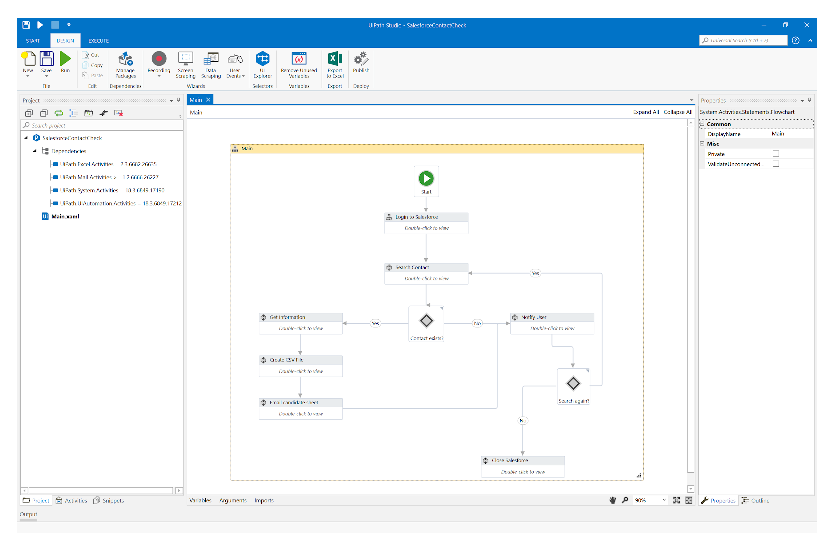
\includegraphics[width=0.8\columnwidth]{chap2/Imagenes/rpauipath.eps}
\caption{Interfaz de usuario de UIPath\cite{Dines2018}.}
\label{fig:uipath}
\end{figure}